\documentclass[prodmode,acmtecs]{acmsmall} % Aptara syntax

\usepackage{amssymb}
\usepackage{amsmath}
\usepackage[margin=1in]{geometry}
\usepackage{exscale}
\usepackage[]{graphicx}
\usepackage[]{graphics}
\usepackage{listings}
\usepackage{float}

% Package to generate and customize Algorithm as per ACM style
\usepackage[ruled]{algorithm2e}
\renewcommand{\algorithmcfname}{ALGORITHM}
\SetAlFnt{\small}
\SetAlCapFnt{\small}
\SetAlCapNameFnt{\small}
\SetAlCapHSkip{0pt}
\IncMargin{-\parindent}

% no indentation - just spaces between paragraphs
\usepackage[parfill]{parskip}

%%%%%%%%%%%%%%%%%%%%%%%%%%%%%%%%%
\setcounter{tocdepth}{2}

\newcommand{\qt}[1]{``#1''}
\newcommand{\code}[1]{\lstinline{#1}}

\lstset{
    language=[ANSI]C,
    basicstyle=\ttfamily,
    tabsize=4
}

%%%%%%%%%%%%%%%%%%%%%%%%%%%%%%%%%

\title{
    Carnegie Mellon University \\
    15-780 Graduate Artificial Intelligence \\
    Final Project: Distributed SLAM
}

\author{
    Adam Wright, Tim Kuehn, \& Nathan Slobody \\
}

\begin{abstract}

We attempt a simple method of combining the results of multiple robots conducting SLAM in an unknown environment with known landmarks.

\end{abstract}

\date{\today}

\begin{document}

\maketitle

\setcounter{tocdepth}{2}

\section{Introduction}

Localization and mapping are fundamental problems in the area of mobile robotics.  For a robot to accomplish a task within an environment, it must have knowledge of the layout of the environment, in the form of a map showing where its goals and obstacles lie.  However, many robotics scenarios involve a robot entering an unknown environment without a map.  Before executing search and planning techniques, it must therefore create a map of the environment and localize itself in that map in order to find its way through and hope to accomplish any goals.  

However, even when the robot has a map, it will not be useful if it is unable to localize itself on that map.  A robot's internal state estimation is thus equally crucial to task completion.

Many real-world applications of robotics, such as search and rescue or indoor fire fighting, do not have the luxury of having an accurate map beforehand. Simultaneous Localization and Mapping (SLAM) techniques, which build maps based only on sensor measurements, allow autonomous robots in these applications to succeed. Further, some applications would benefit from using multiple robots to cover a wide area quickly.

In this project, we implement a simple system for distributed SLAM using multiple robots in simulation.  These robots perform SLAM individually and share their data to create a larger combined map of the area.

\section{Background}

\subsection{SLAM}

The idea behind SLAM is to use a probabilistic method to solve mapping and localization as a single problem.  Mapping and localization are typically both attempted under conditions of sensor noise and uncertain state estimation.  SLAM techniques take advantage of the idea that feedback from both processes can reinforce each other at each step of an iterative state estimation; in fact, SLAM's model states that it is impossible in practice to separate the two.

Since, in theory, accurate localization can not be achieved without an accurate map on which to localize, and an undistorted map cannot be created without an accurate statement of present localization, the SLAM problem is iterative in practice.  Starting conditions converge towards better estimates of both over time and subsequent observations.

SLAM is an active research topic with a number of current approaches, including several varieties of Kalman filtering (linear, extended, unscented), particle filtering, smoothing, and others.  The implementation we chose is based on a linear Kalman filter.

\subsection{Kalman Filter}

The Kalman filter is a Bayesian method of updating prior predictions based on current observations.  The assumptions underlying the linear Kalman filter are that the underlying system has fundamentally linear dynamics and that errors are normally distributed.

At a high level the Kalman filter involves a transition model describing the relationship between a state at two consecutive timesteps $x_t$ and $x_{t+1}$, and a measurement model describing the relationship between what is perceived and the system state at a given timestep.

The transition model is given by:
\begin{align*}
    x_t' &= F x_t + G u_t + \nu_t \\
\end{align*} 

where $\nu_t$ is gaussian noise with covariance matrix $Q$.

The measurement model is given by:

\begin{align*}
    Z_k &= H_k x_k + w_k
\end{align*}

where $w_k$ is gaussian noise with covariance matrix $R$.

The Kalman filter involves two steps: predict and update. In the prediction step, given by:

\begin{align*}
    x_t' &= F x_t + G u_t \\
    P_t' &= F P F^T + Q
\end{align*}

the filter produces estimates of current state variables with associated uncertainties.

In the update step, given by:

\begin{align*}
    y &= z_t - H_t x_t' \\
    S &= H_t P_t' H^T_t + R_t \\
    K &= P_t' H^T_t S^{-1} \\
    x_{t+1} &= x_t' + Ky \\
    P_{t+1} &= (I - K H_t) P_t'
\end{align*}

the algorithm averages the current observations against prior predictions, giving more weight to estimates with higher certainty.

The matrix definitions are as follows:

\begin{align*}
    x:& \text{ System state}\\
    H:& \text{ Motion model}\\
    P:& \text{ Covariance matrix}\\
    R:& \text{ Measurement uncertainty}\\
    Q:& \text{ Motion covariance / uncertainty}
\end{align*}

$x$, the system state, describes the present estimates of the robot's location and any landmarks that it has seen to date.

$H$ describes the assumption of the perception model that maps the true space into the observation space.

$P$ is the covariance of the uncertainty in state estimation parameters.

$R$ is the uncertainty or error in sensing.

$Q$ is the uncertainty in motion.


\section{Model}

The problem that our model addresses is that of a robot entering an unknown area but searching for known landmarks within it.  However, while it is able to recognize the landmarks upon sensing them, it still does not know what their absolute positions are \- only the positions relative to itself and what it has already mapped.

For analogy, consider a person walking into the Louvre museum without a map.  He does not know much about art and doesn't know where any paintings are within the museum.  However, he knows what the famous ones look like and when he sees the Mona Lisa he recognizes it immediately. If he has been tracing his steps from the beginning, can give a position for the painting relative to the museum's entry point.  If he later comes across the Venus de Milo, he can relate its position to both the Mona Lisa and his entry point.  (Of course, if he daydreamed while walking to the Mona Lisa and wasn't sure about how many steps he actually took, all of the relative positions will be slightly off.)

This is similar to the model we are exploring here, with the Louvre standing in for an unknown area, the famous artworks being landmarks, and the robot daydreaming representing an odometry error.  It could be applicable to a variety of robotic exploration scenarios; for instance, search-and-rescue operations.

In order to focus on the main problem, we abstracted away certain details in our simulation.  In particular, we assume that when a robot senses a known landmark, it can identify it immediately and without error.  Normally there would be some uncertainty involved in, say, a vision sensor identifying visual features, but for simplicity we did not consider this in our model.

In addition, our motion and sensor models are simplified as described in the next section.

\section{Implementation}

We assume a simple linear system with gaussian transition and sensor noise.  Covariance matrices express relationships between landmarks and robot positions and between landmarks themselves.  

We utilized Python and NumPy and for our numerical calculations and the Tkinter graphical framework to visualize our simulation.

Figure~\ref{fig:simulation} shows a screenshot of the simulation.  The rectangles are robots, and the lines coming out of them represent the extent of their sensors.  The black circles represent unique landmarks.  The blue and red circles around or inside landmarks are the robots' estimations of where the landmarks are; the size of the circle represents its uncertainty about the landark's exact position, with a larger circle representing more uncertainty.

\begin{figure}[h!]
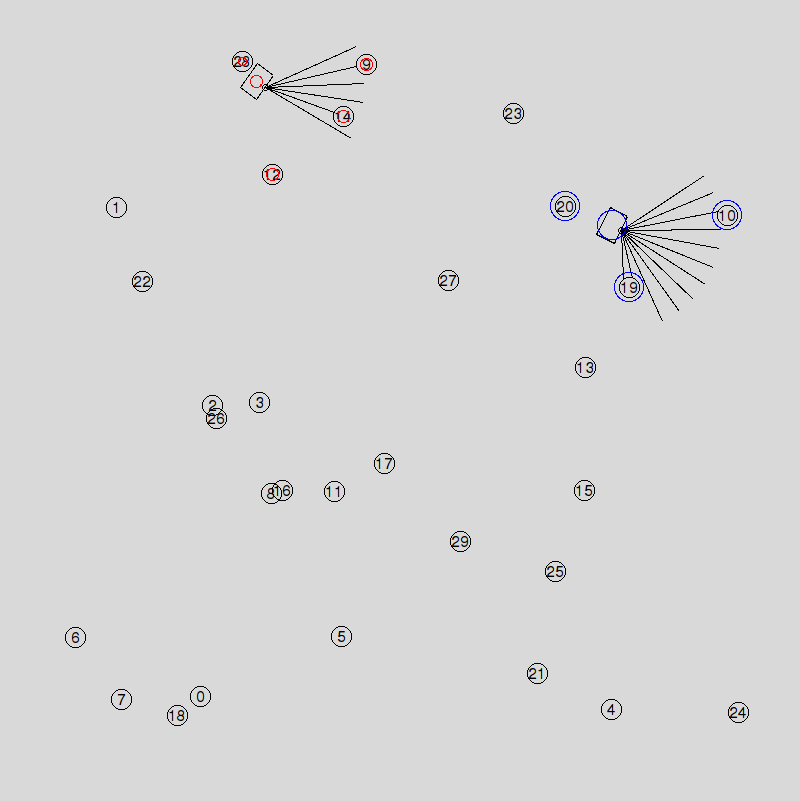
\includegraphics[width=\textwidth]{screenshot.png}
\caption{Simulation environment.}
\label{fig:simulation}
\end{figure}

The blue and red circles on the robots themselves represent the robots' estimation and uncertainty about their own position.

A diagram of the system is shown Figure~\ref{fig:system}.

\begin{figure}[h!]
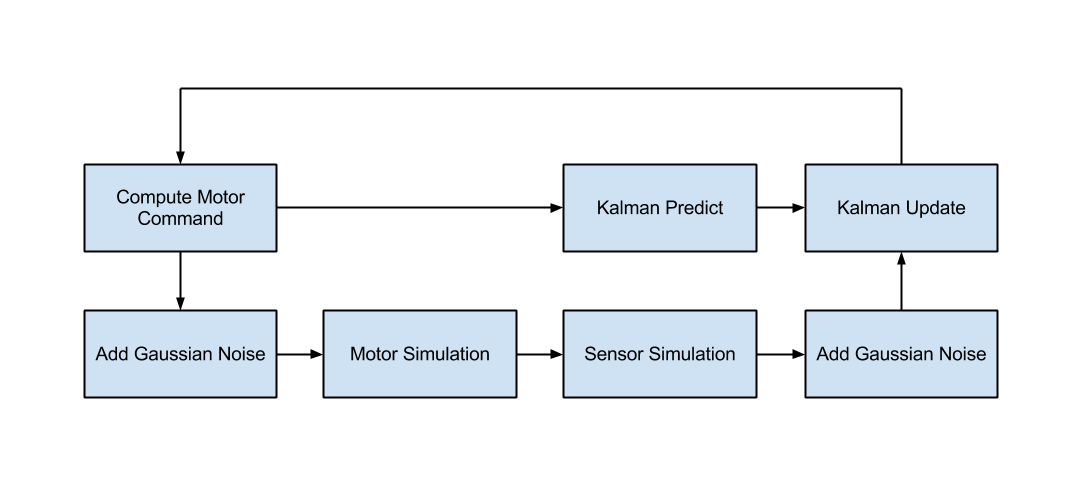
\includegraphics[width=\textwidth]{systemdiagram.png}
\caption{The flow of the program.}
\label{fig:system}
\end{figure}

\subsection{Parameters}

Since the robot starts out not knowing about any landmarks, and adds new landmarks to its database at every time step, we must recompute all the matrices in our model at every timestep. The system state, $x$ is
$$
x 
= 
\begin{bmatrix}
    x_r \\
    y_r \\
    \theta_r \\
    x_{a_1} \\
    y_{a_1} \\
    \vdots \\
    x_{a_n} \\
    y_{a_n} \\
\end{bmatrix}
$$

Where $[x_r, y_r, \theta_r]^T$ is the robot's pose, and $[x_i, y_i]^T$ is landmarks $i$'s $x$ and $y$ location, and $\{a_1,\ldots,a_n\}$ is the ordering of the landmarks in the $x$ vector. This ordering is dependent on the order in which landmarks are discovered by the robot. All locations are in the global reference frame. The estimate of $x$ may be referred to as $\hat{x}$.

P is the covariance of the state estimate. $\hat{x}$ and $P$ are the parameters of the multivariate distribution that describes the current estimate of the system state.

$$
P =
\begin{bmatrix}
    var(x_r)     & 0            & 0               & cov(x_r,x_1) & 0            & cov(x_r,x_2) & 0            \\
    0            & var(y_r)     & 0               & 0            & cov(y_r,y_1) & 0            & cov(y_r,y_2) \\
    0            & 0            & var(\theta)     & 0            & 0            & 0            & 0            \\
    cov(x_r,x_1) & 0            & 0               & var(x_1)     & 0            & cov(x_1,x_2) & 0            \\
    0            & cov(y_r,y_1) & 0               & 0            & var(y_1)     & 0            & cov(y_1,y_2) \\
    cov(x_r,x_2) & 0            & 0               & cov(x_1,x_2) & 0            & var(x_2)     & 0            \\
    0            & cov(y_r,y_2) & 0               & 0            & cov(y_1,y_2) & 0            & var(y_2)     \\
\end{bmatrix}
$$

The diagonals of this matrix are just the variances of each variable in the state vector. The off-diagonal elements are the covariances between different variables in the vector. There are few elements of the matrix that are used to express relationships between variables in the state. Whenever a landmark is seen for the first time, it is appended to the state estimate, and the variance of that landmark's $x$ and $y$ positions are inserted at the bottom right of the covariance matrix. We also add some covariance between the robot's pose and the landmark position, where appropriate. For example, if the robot observed landmark $1$, and it had not seen any landmarks before, the state would become

$$
x
=
\begin{bmatrix}
    x_r \\
    y_r \\
    \theta_r \\
\end{bmatrix}
\Rightarrow
\begin{bmatrix}
    x_r \\
    y_r \\
    \theta_r \\
    x_1 \\
    y_1 \\
\end{bmatrix}
$$

and the covariance matrix would become

$$
P
=
\begin{bmatrix}
    var(x_r)     & 0            & 0               \\
    0            & var(y_r)     & 0               \\
    0            & 0            & var(\theta)     \\
\end{bmatrix}
\Rightarrow
\begin{bmatrix}
    var(x_r)     & 0            & 0               & cov(x_r,x_1) & 0            \\
    0            & var(y_r)     & 0               & 0            & cov(y_r,y_1) \\
    0            & 0            & var(\theta)     & 0            & 0            \\
    cov(x_r,x_1) & 0            & 0               & var(x_1)     & 0            \\
    0            & cov(y_r,y_1) & 0               & 0            & var(y_1)     \\
\end{bmatrix}
$$

Since the components of the robot and landmark positions are related. That is, if the robot has $x$ position $x_r$ at time $t$ and the landmark has $x$ position $x_1$, then the two quantities are related because the robot was at a specific distane from landmark 1 at time $t$.

\subsection{Motion Model}

We also have the motion command, where $u=[\Delta x_r, \Delta y_r, \Delta \theta_r]^T$, or the change robot pose from timestep $t$ to timestep $t+1$.

For our transition model, we set $F$ to be the identity matrix of the appropriate size. Thus our transition model becomes $x_{t+1} = x_t + G_tu_t + \nu_t$. An example of our transition model for one timestep follows. In this example the robot has already observed landmark 1, and has an estimate of that landmark's position in its state: $x_t=[3, 4, \pi, x_1, y_1]^T$, and $u_t = [1,1,0]^T$. In this case the transition model equation will look like this:

$$
\begin{bmatrix}
    4  \\
    5  \\
    \pi\\
    30 \\
    40 \\
\end{bmatrix}
=
\begin{bmatrix}
    3  \\
    4  \\
    \pi\\
    30 \\
    40 \\
\end{bmatrix}
+
\begin{bmatrix}
    1 & 0 & 0  \\
    0 & 1 & 0  \\
    0 & 0 & 1  \\
    0 & 0 & 0  \\
    0 & 0 & 0  \\
\end{bmatrix}
\begin{bmatrix}
    1 \\
    1 \\
    0 \\
\end{bmatrix}
$$

The purpose of $G$ in this model is simply to convert $u_t$ into an $n\times 1$ matrix, where $n$ is the size of $x$, so the change in pose is added to the proper elements in $x$.

The last part of the motion model is the system noise covariance, $Q$. We define $Q$ as follows:

$$
Q = 
\begin{bmatrix}
    cov(\Delta x_r) & 0               & 0 \\
    0               & cov(\Delta y_r) & 0 \\
    0               & 0               & cov(\Delta \theta_r) \\
\end{bmatrix}
$$

This takes into account the fact that our robot may not move exactly how it expects to move when it executes a motor command. The variances on the diagonal are set to be a 5\% of the attempted motion.

\subsection{Measurement Model}

Since our measurements are relative position between the motors and the landmarks, the $H$ matrix in the measurement model must express that. The relative sensor measurement is

$$
z = 
\begin{bmatrix}
    x_{a_1} - x_r \\
    y_{a_1} - y_r \\
    \vdots\\
    x_{a_m} - x_r \\
    y_{a_m} - y_r \\
\end{bmatrix}
$$ 

where $\{a_1,\ldots,a_m\}$ is the list of landmark ids that were measured at timestep $t+1$. An example of our measurement model, if the robot discovered landmarks in the order $\{1,4,2\}$, and has estimates of them in its state, a relative measurement of landmarks 1 and 2 would look like this:

$$
\begin{bmatrix}
    x_1 - x_r \\
    y_1 - y_r \\
    x_2 - x_r \\
    y_2 - y_r \\
\end{bmatrix}
=
\begin{bmatrix}
    -1 & 0 & 0 & 1 & 0 & 0 & 0 & 0 & 0 \\
    0 & -1 & 0 & 0 & 1 & 0 & 0 & 0 & 0 \\
    -1 & 0 & 0 & 0 & 0 & 0 & 0 & 1 & 0 \\
    0 & -1 & 0 & 0 & 0 & 0 & 0 & 0 & 1 \\
\end{bmatrix}
\begin{bmatrix}
    x_r \\
    y_r \\
    \theta_r \\
    x_1 \\
    y_1 \\
    x_4 \\
    y_4 \\
    x_2 \\
    y_2 \\
\end{bmatrix}
$$

This $H$ matrix properly computes the relative measurement from the state's absolute positions.

The final piece of the measurement model is the covariance matrix of the measurement noise $w$, $R$. We set $R$ such that the variances of the relative landmark measurements are equal to our approximate sensor error, which is about 5\% of the max sensor range. So the for a measurement

$$
z
=
\begin{bmatrix}
    x_1 \\
    y_1 \\
    x_2 \\
    y_2 \\
\end{bmatrix}
$$

we would have the covariance matrix

$$
R
=
\begin{bmatrix}
    var(x_1)     & 0            & cov(x_1,x_2) & 0            \\
    0            & var(y_1)     & 0            & cov(y_1,y_2) \\
    cov(x_1,x_2) & 0            & var(x_2)     & 0            \\
    0            & cov(y_1,y_2) & 0            & var(y_2)     \\
\end{bmatrix}
$$

to express that landmark $x$ and $y$ values are related, just as robot $x$ and $y$ values are related to landmarks.

\subsection{Distributed SLAM}

The most basic approach to distributed SLAM is to assume that communication is always on, and just propagate all measurements and motion commands to every robot. This is simple, but can be computationally expensive, and wastes a lot of compute on each robot combining the same measurements into different covariance matrices. This technique works fine when communication is perfect, but imagine communication is not perfect and robots can only talk to a small group of other robots. Now each group can combine their measurements and motor commands, but we cannot ever take the measurements we made at this timestep and apply them other robots that are out of our group.

We consider another approach, which users another Kalman filter to fuse the robots' data. The transition model would copy over the pose of each robot into the right place in the combined state vector, and the measurement model would treat the each robot's state as a measurement. The $H$ matrix in the measurement model would look something like

$$
H
=
x 
= 
\begin{bmatrix}
    x_1    \\
    y_1    \\
    \vdots \\
    x_m    \\
    y_m    \\
\end{bmatrix}
=
\begin{bmatrix}
    [ 0 ]  & [ 0 ]  & [ 1 ] & [ 0 ] & [ 0 ]  & [ 0 ]  & [ 0 ]  & [ 0 ] \\
    [ 0 ]  & [ 0 ]  & [ 0 ] & [ 1 ] & [ 0 ]  & [ 0 ]  & [ 0 ]  & [ 0 ] \\
    [ 0 ]  & [ 0 ]  & [ 0 ] & [ 0 ] & [ 1 ]  & [ 0 ]  & [ 0 ]  & [ 0 ] \\
    \vdots & \vdots & \vdots & \vdots & \vdots & \vdots & \vdots & \vdots \\
    [ 0 ]  & [ 0 ]  & [ 0 ] & [ 0 ] & [ 0 ]  & [ 0 ]  & [ 1 ]  & [ 0 ] \\
    [ 0 ]  & [ 0 ]  & [ 0 ] & [ 0 ] & [ 0 ]  & [ 0 ]  & [ 0 ]  & [ 1 ] \\
\end{bmatrix}                 
\begin{bmatrix}
    [ r_1 ] \\
    [ r_2 ] \\
    \\
    [ l_1 ] \\
    \vdots \\
    [ l_m ] \\
\end{bmatrix}
$$

where there are only 2 robots, $[1]$ indicates an identity matrix of size $2\times 2$ and $[0]$ indicates a $2\times 2$ 0 matrix. This model design ensures that the Kalman filter updates any landmark measurements and related robot poses.

\section{Results}

\subsection{Individual Robots}

Individual robots are able to perform SLAM reliably.  When sensing a new landmark, a robot adds the landmark to its list of those encountered with an initial estimation of its location, relative to its own.  This estimate improves as the robot encounters other nearby landmarks, and continues to improve if the robot returns to perceive the landmark again.

The robot's estimation of its own position is partly a function of the uncertainty encoded into the odometry.  With a reasonable level of odometry error, the robot gradually loses track of its position over time if it travels a distance without sensing any landmarks, which is the expected result. This effect is shown in Figure \ref{fig:waypoints}, with the robot having low uncertainty (signified by the thickness of the trail) when it is within range of landmarks, and high uncertainty when it cannot see landmarks. When the robot sees a new group of landmarks again, they appropriately off due to the cumulative error of the robot.

\begin{figure}[h!]
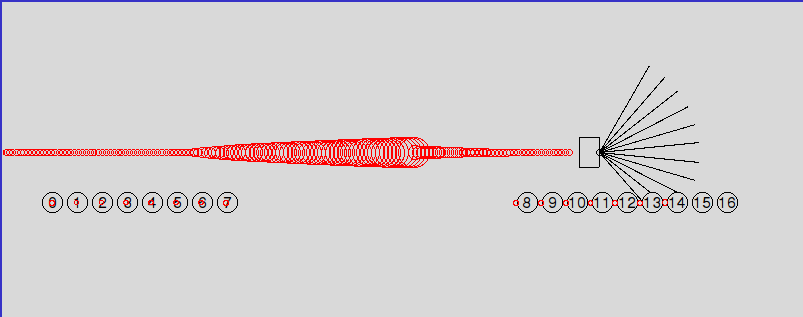
\includegraphics[width=\textwidth]{waypoints.png}
\caption{Cumulative error increases uncertainty unless landmarks can be measured.}
\label{fig:waypoints}
\end{figure}

\begin{figure}[h!]
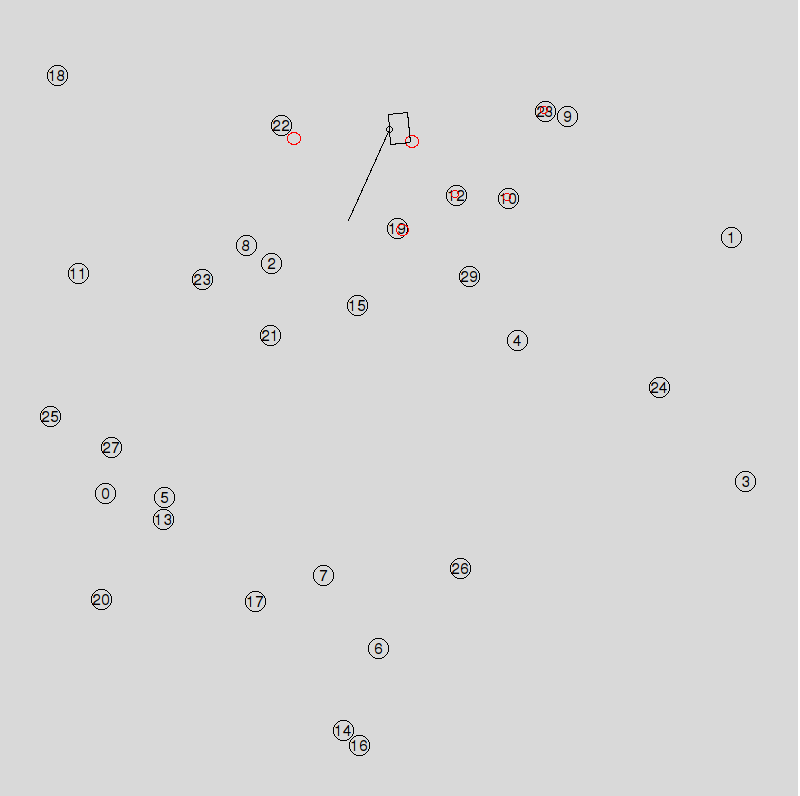
\includegraphics[width=\textwidth]{update1.png}
\caption{After sensing a new landmark for the first time.  The robot's incomplete sight lines are an artifact of screen flicker.}
\label{fig:update1}
\end{figure}

These results can be seen in Figures~\ref{fig:update1} and~\ref{fig:update2}.  In Figures~\ref{fig:update1}, the robot has observed several previous landmarks and traveled a small distance away from them where it has observed landmark 22.  The previously-observed landmarks appear with a high degree of certainty in their position estimate.  However, due to odometry error while traveling through landmark-free space, the robot has slightly lost track of its current position, and when it encounters landmark 22, its prediction of its relative location is off by the same error factor.

\begin{figure}[h!]
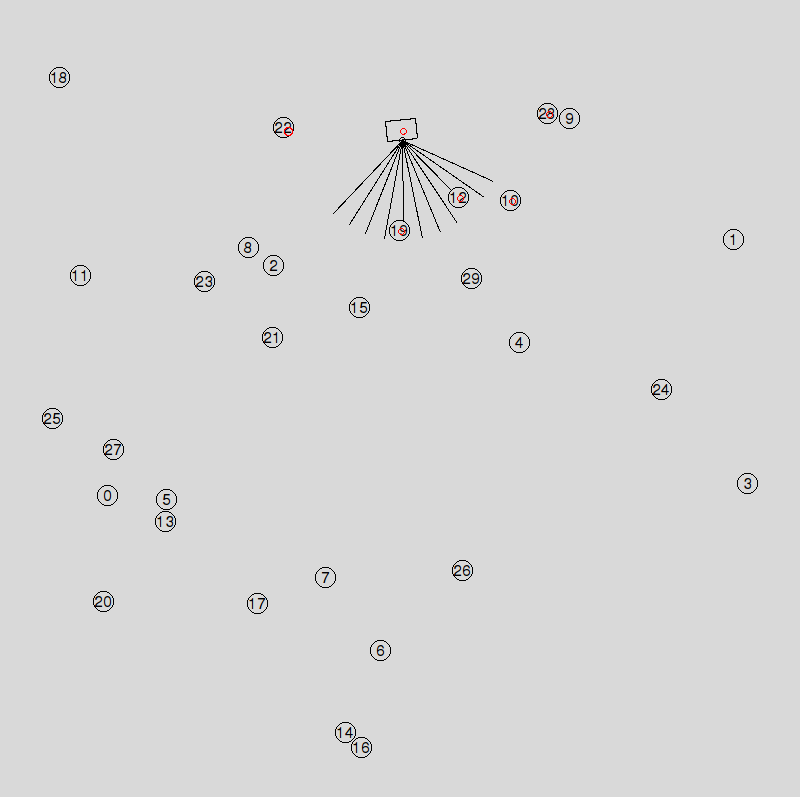
\includegraphics[width=\textwidth]{update2.png}
\caption{After returning to previously observed landmarks.}
\label{fig:update2}
\end{figure}

In Figures~\ref{fig:update1}, the robot has moved back toward landmarks that it had observed previously (numbers 12 and 19).  Once it makes a new observation of these landmarks, both its estimate of its current location and its estimate of landmark 22's location become more accurate, and with higher certainty.

One problem we encountered was with numerical instability.  When setting the uncertainty matrices to levels at or near zero, the robots' measurements tended to become unreliable.  

\subsection{Multiple Robots}

Multiple robots working in the same area individually are able function without problems, but joining their results into a distributed framework has proven to be less successful so far.

\section{Future Work}

In addition to fine-tuning the distributed aspect of the project, we would like to apply our implementation to real robots in a real environment.

\begin{thebibliography}{12}
    \bibitem{thrun2005}
        S. Thrun, W. Burgard, and D. Fox, \emph{Probabilistic Robotics}, MIT Press, 2005.

    \bibitem{thrun2003}
        S. Thrun and Y. Liu, ``Multi-Robot SLAM with Sparse Extended Information Filters'', \emph{Proceedings of the 11th International Symposium of Robotics Research (ISRR'03)}, 2003.

    \bibitem{cunningham2010}
        A. Cunningham, M. Paluri, and F. Dellaert, ``DDF-SAM: Fully Distributed SLAM using Constrained Factor Graphs'', \emph{International Conference on Intelligent Robots and Systems (IROS)}, 2010.
\end{thebibliography}

\end{document}
